\documentclass[10pt, conference, letterpaper]{IEEEtran}
\usepackage{mathbbold}
\usepackage{amsfonts}
\usepackage{}
\usepackage{latexsym,bm,amsmath,amssymb}
\usepackage{cite}
\usepackage{algorithm}
\usepackage{multirow}
\usepackage{algorithmic}
\usepackage{graphicx}
\usepackage{subfigure}
\usepackage{color}
\usepackage{balance}

\newtheorem{theorem}{\textbf{Theorem}}
\newtheorem{definition}{\textbf{Definition}}
\newtheorem{lemma}{\textbf{Lemma}}
\newtheorem{Proof}{\textbf{Proof}}
\newtheorem{problem}{\textbf{Problem}}
\renewcommand{\thefootnote}{\fnsymbol{footnote}}
\renewcommand{\algorithmicrequire}{ \textbf{Input:}} %Use Input in the format of Algorithm
\renewcommand{\algorithmicensure}{ \textbf{Output:}} %UseOutput in the format of Algorithm
% correct bad hyphenation here
\hyphenation{op-tical net-works semi-conduc-tor}


\begin{document}

\title{Attention-based Sign Language Recognition via Multisensor Fusion}
%DeepSLR: A Deep Learning Approach for Sign Language Recognition via Multisensor Fusion

%author names and affiliations

%\author{\IEEEauthorblockN{Zhibo Wang$^{\dagger,\ddagger,\wr}$, Yongquan Zhang$^{\dagger}$, Honglong Chen$^{\pounds}$, Zhetao Li$^{\P,\ast}$\footnotetext[1], and Feng Xia$^{\S}$}
%\IEEEauthorblockA{$^{\dagger}$School of Cyber Science and Engineering, School of Computer, Wuhan University, P. R. China}
%\IEEEauthorblockA{$^{\ddagger}$Jiangsu Key Lab. of Big Data Security \& Intelligent Processing, NJUPT, P. R. China}
%\IEEEauthorblockA{$^{\wr}$Key Lab of Aerospace Information Security and Trusted Computing, Wuhan University, P. R. China}
%\IEEEauthorblockA{$^{\pounds}$College of Information and Control Engineering, China University of Petroleum, P. R. China}
%\IEEEauthorblockA{$^{\P}$College of Information Engineering, Xiangtan University, P. R. China}
%\IEEEauthorblockA{$^{\S}$School of Software, Dalian University of Technology, P. R. China}
%Email: \{zbwang, dellenzhang\}@whu.edu.cn, \{honglongchen1984, liztchina\}@gmail.com, f.xia@ieee.org}
\maketitle
%\footnotetext[1]{Corresponding author.}


\begin{abstract}
Nowadays, tens of millions of deaf and mute people around the world use sign language for daily communication, whereas most ordinary people have little knowledge of sign language. Therefore, we need an effective method of Sign Language Recognition (SLR) to help bridge the communication gap between hearing impaired people and ordinary people. Existing SLR methods are generally based on vision signals (e.g., video cameras, infrared cameras), acoustic signals, optic signals, radio frequency. However, these solutions use only one or two types of sensors to build their SLR models. They often neglected the multi-level, multi-space information complementation and combinatorial optimization processing of multiple sensors. In addition, existing SLR methods generally have poor performance in identifying continuous sentences without word by word segmentation. 

In this paper, we adopt an inertial measurement unit (IMU) sensor and a multichannel surface electromyogram (sEMG) sensor to collect multi-level raw data of two-hand sign language motions. Furthermore, we propose a novel SLR framework: attention-based SLR (AttentionSLR). Instead of using word by word segmentation, it can continuously translate sign language motions into sentences based on words. AttentionSLR consists of three components: multi-level feature extraction, multi-level feature fusion, and the attention model of SLR. Experiment....

\end{abstract}

\IEEEpeerreviewmaketitle

\section{Introduction}
The number of people who use sign language is impressive. In fact, there are approximately 28 to 32 million deaf and hard of hearing people living in the USA \cite{population.org}, and there are roughly 65 to 70 million hearing-impaired people in the world. In addition, people who use sign language also include sign language lovers and workers from special education and government service departments. To better help hearing-impaired people and communicate with the huge amount of sign language users, an effective and convenient method is required. 

Sign language recognition (SLR), which is an effective method to bridge the communication gap, aims to translate a series of sign language motions to a sentence based on words. However, SLR is more delicate and complex compared with other gesture recognition. Because sign language is composed of a specific set of fine-grained finger motions and coarse-grained arm movements. Most existing research has attempted to acquire sign language data through one or two types of sensors. However, sensors of these methods usually suffer from the lack of robustness, integrity, and convenience. The approaches using video or infrared cameras \cite{huang2018video,neto2018sign,joshi2017personalizing,cui2017recurrent,tsironi2016gesture,dong2015american} fail to recognize gestures in poor lighting conditions. There are approaches using microphones to collect data \cite{mao2016cat,nandakumar2016fingerio}. Although microphones are lightweight devices, they are sensitive to the noise in real-world environment. The approach based on photoplethysmography (PPG) \cite{zhao2018ppg} cannot guarantee the integrity of SLR, because it can only recognize fine-grained finger motions and lacks a key component of the sign language: the trajectory of coarse-grained arm movements. The approaches based on radio frequency (RF) \cite{zhang2017doppler,sun2015widraw,pu2013whole,asadzadeh2012gesture} usually require very bulky equipment and extra manpower of installation. The approaches using sensing gloves require the user to wear a pair of gloves to capture sign language gestures \cite{swee2007wireless,mantyjarvi2004enabling,mehdi2002sign}. However, the gloves, which are cumbersome, may become a burden for users and even result in mental stress. Additionally, most approaches recognize sign language using word by word segmentation, or just do the recognition of a single sign language motion. The difficulty of active segmentation generally limits their performance in continuous SLR.
\begin{figure}[!t]
  \centering
  \vspace{-3mm}
  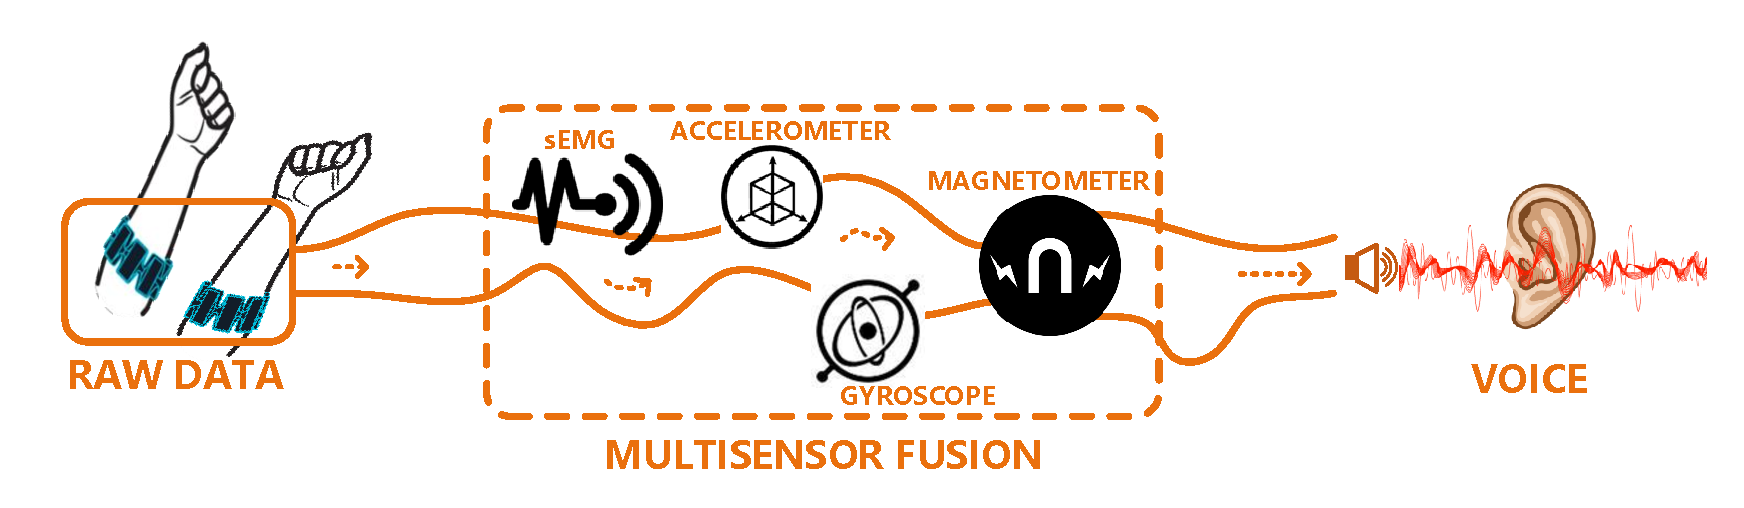
\includegraphics[width=1.0\columnwidth]{pics/1.pdf}
  \caption{Illustration of the our attention-based continuous SLR model.}
  \label{fig:highlevel}
\end{figure}
\vspace{-1mm}

In order to address the problems above, we decided to design a continuous SLR framework based on multi-sensor. Multi-sensor offers a robust, integrated, and convenient way of collecting the data of sign language. And the continuous recognition makes sure the practicality of our SLR framework. There are following challenges need to be addressed. 
\begin{itemize}
\item A key challenge is building a multi-sensor system that can reliably and conveniently capture both fine-grained finger motions and coarse-grained arm movements.
\item Due to the diversity and complexity of our input data, an effective method is required to extract the multi-level feature from the data.
\item Improving the performance of continuous SLR, which has not been thoroughly studied, is the main challenge.
\end{itemize} 

In this paper, we adopted two MYO \cite{timmurphy.org} armbands to collect multi-level raw data of two-hand sign language motions. Instead of using word by word segmentation, we then proposed a attention-based continuous SLR model named AttentionSLR. AttentionSLR is composed of multi-level feature extraction, multi-level feature fusion and the attention model of SLR. As illustrated in Figure \ref{fig:highlevel}, AttentionSLR translates the multi-sensor data (sEMG signal, gyroscope signal, acceleration signal, magnetometer signal) collected from a user's forearms into sentences based on words. 

To be specific, a MYO armband is composed of an inertial measurement unit (IMU) sensor and a multichannel surface electromyogram (sEMG) sensor. Electromyographic (EMG) signals are the temporal and spatial superposition of motor unit action potentials (MUAP) in muscle fibers. The sEMG sensor captures the combined signal of superficial muscle EMG and the neural stem activity on the surface of skin, which can effectively reflect neuromuscular activity. And the IMU sensor consists of a precision gyroscope (GYRO), an accelerometer (ACC), and a magnetometer (MAGN) in a multi-axis fashion. sEMG and IMU sensor respectively captures the fine-grained finger motions and the coarse-grained arm movements of a user. Besides the data integrity, the armband is also stable and convenient to wear.

Extraction of IMU and EMG features have been considered in the literature \cite{kosmidou2006evaluation, khushaba2007channel, mantyjarvi2004enabling, kela2006accelerometer}. Owing to the complexity of our data, we proposed a novel multi-level feature extraction algorithm in AttentionSLR. We first used wavelet transform (WT) to reduce the noise in our data. Then we designed a multi-stream convolutional neural network (CNN) to extract the temporal features of our data. Finally, the extracted features were represented as vectors.

To achieve continuous SLR, we proposed a multi-level feature fusion approach and designed the attention-based model for recognition. The features we extracted from the raw data along with quaternion, which is an extra feature calculated from IMU signals, will be used as the input of our feature fusion multi-layer perceptron (MLP). Intuitively, our MLP maps the high-dimensional input to a low-dimensional embedding. Our attention-based network consists of 
the two-stream long-short term memory (LSTM) encoder and decoder and an attention layer. By using the embedding as the input, our attention model decodes the input to a sentence word by word. The main contributions of our paper are summarized as follows:
\begin{itemize}
  \item A multi-sensor data collector system that can reliably and conveniently capture both fine-grained finger motions and coarse-grained arm movements.
  \item A new method to extract the multi-level feature from the complex sign language signals.
  \item An effective approach of multi-level sign language feature fusion.
  \item A attention-based model for continuous SLR without word by word segmentation.
\end{itemize}

The rest of the paper is organized ad follows. We discuss the relate work in Section II.

\section{Related Work}
\label{sec:related_work}
%In this section, a brief review of current techniques for SLR and continuous SLR.
According to the technology used to capture gestures, traditional gesture recognition studies can be divided into the following categories: vision-based, acoustic-based, optic-based, RF-based, and biosensor-based.

\vspace{1mm}
\textbf{Vision Based:} Computer vision-based methods can effectively track and recognize gestures through the camera \cite{huang2018video,neto2018sign,joshi2017personalizing,cui2017recurrent,tsironi2016gesture,ren2016robust,dong2015american,marin2014hand}. While, these research methods are very sensitive to the environment such as illumination, background texture and color \cite{mitra2007gesture,mantyjarvi2004enabling}. In order to improve the accuracy and robustness of vision-based methods, some previous studies
took advantage of  colored gloves \cite{starner1998real} or multiple cameras \cite{vogler1998asl} for accurate hand gesture tracking, segmentation, and recognition \cite{zhang2011framework}.

\textbf{Acoustic Based:} Acoustic-based \cite{mao2016cat,nandakumar2016fingerio} approaches can acquire gesture information through speakers and microphones. Nevertheless, the sound signals in our actual use environment are strongly noisy, and the ambient noise decibels tend to be much higher than the information about the dynamics of the gestures.

\textbf{Optic Based:}Optic-based \cite{zhao2018ppg,li2015human} methods require specific light sensor devices. Moreover, which cannot achieve complete SLR. Because complete sign language includes fine-grained finger movements and coarse-grained gesture trajectories, it \cite{zhao2018ppg} only achieves finger-level recognition.

\textbf{RF Based:}RF-based SLR has received much attention from many scholars. For example, Zhang \cite{zhang2017doppler} propose to use Doppler-Radar (DR) and CNN to achieve symbol recognition. In addition, some others use the multi-path effects of Frequency-Modulated Continuous-Wave (FMCW) \cite{adib2015multi,adib20143d} signals, channel state information (CSI) \cite{sun2015widraw,pu2013whole} and the Universal Software Radio Peripheral (USRP) in the environment for SLR. However, these methods require a certain amount of space and dedicated equipment to ensure experimental results, so they are not practical.

\textbf{Body Sensor Based:}Some previous studies based on body sensors have used sEMG sensors \cite{kosmidou2006evaluation,lu2014hand}, or Electrical Impedance Tomography (EIT) \cite{zhang2015tomo} sensors or electrocardiogram (ECG) \cite{zhang2011framework} sensors alone to obtain gesture information. A step further, there are also some ways to combine EMG signal and accelerometer(ACC) signal to obtain gesture information. But they ignore the very important point that the composition of sign language movements is very complicated. The EMG signal can only represent the activity of the finger, and the ACC signal can only represent some simple gesture trajectories on the horizontal and vertical axes. The attitude calculation cannot be completed by the acceleration sensor alone.

Different from previous work, we propose a approach of multi-information fusion in the recognition of two-hand sign language. The 8-channel medical sEMG sensor captures fine-grained finger movements. High sensitivity 9-axis IMU sensor (i.e., triaxial gyroscope, triaxial accelerometer and triaxial magnetometer) captures coarse-grained gesture movements. The sEMG signal represents fine finger movement. The acceleration signals changing with time can directly represent patterns of hand gesture trajectories. The gyroscope can directly represent the rotation mode of the arm by measuring its own rotation transformation. The magnetometer can orient the arm (east, north, south, and north) and modify the static cumulative error of the gyroscope. Therefore, in our system, due to error correction and error compensation, it is often combined with the above sensors to make full use of the characteristics of each sensor to make the final calculation result more accurate. What's more, The Euler angle (EULA) can be calculated by a MAGN and an ACC. In order to avoid the problem of the gimbal deadlock, we can calculate the quaternion from the EULA. Latent space model is a popular tool to bridge the semantic gap between two modalities




\vspace{1mm}

\section{System Overview and Problem Formulation}
\label{sec:problem}
In this section, we first present the high-level overview of attention-based continuous SLR systems without word by word segmentation via multisensor fusion, and then describe the multi-source information fusion design problem and the continuous sentence recognition problem.

\begin{figure*}[!ht]
  \centering
  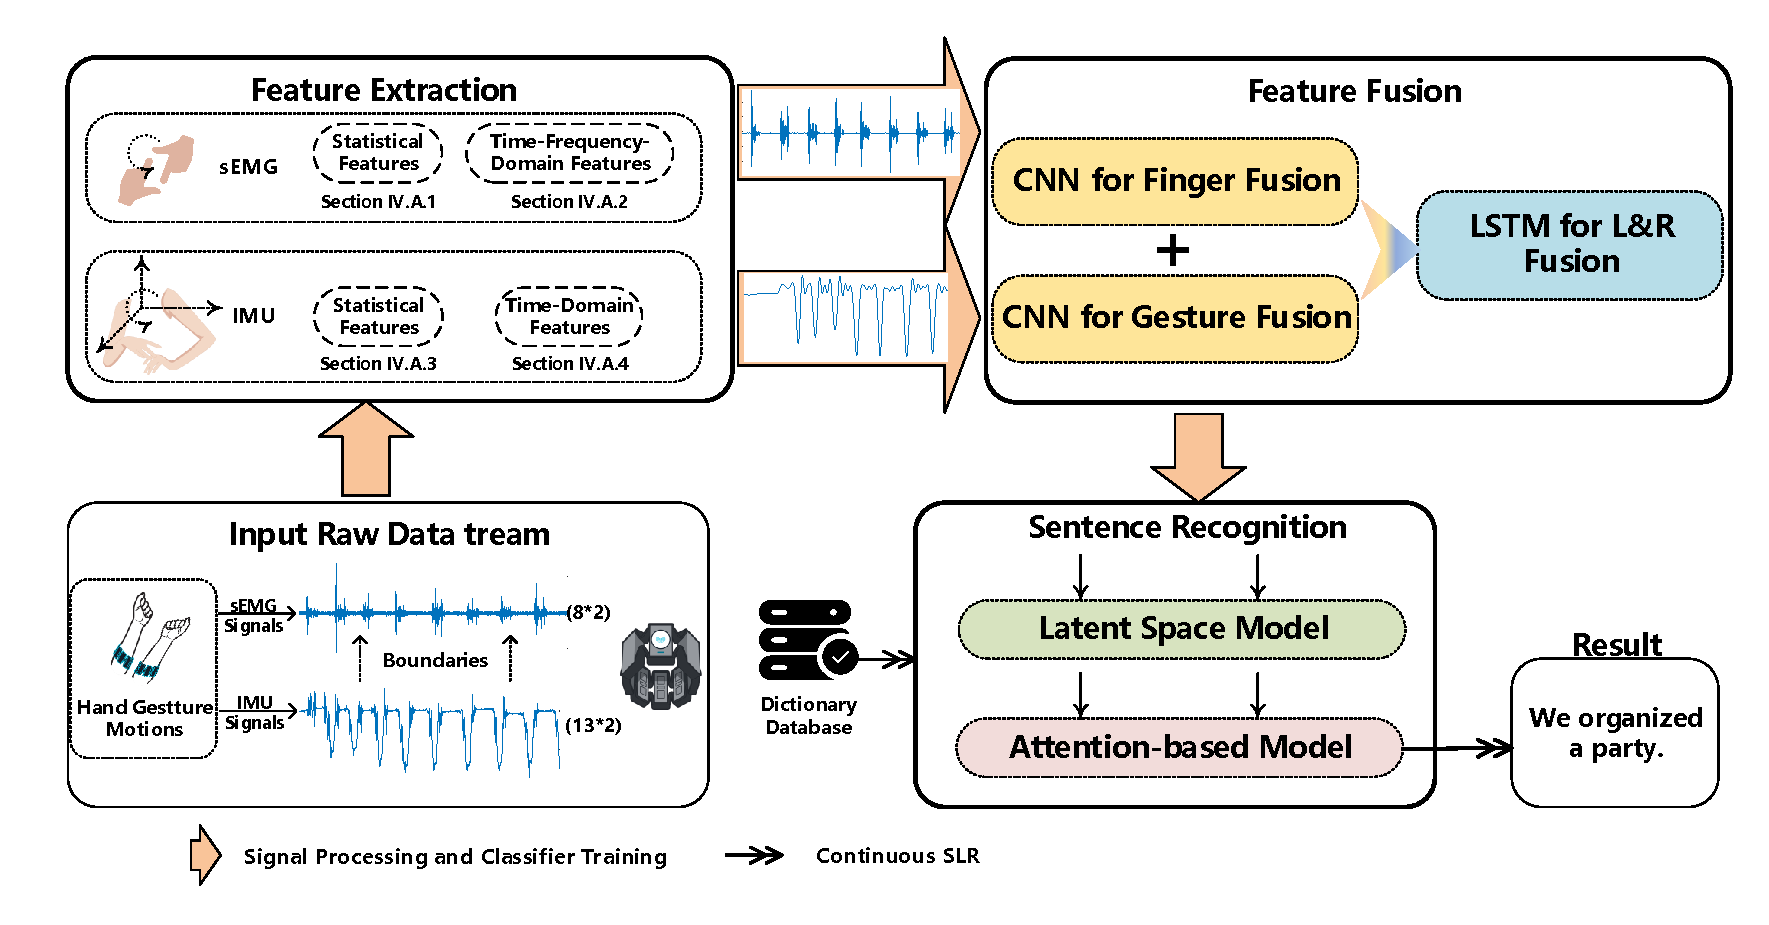
\includegraphics[width=0.9\textwidth]{pics/SystemOverview.pdf}
  \caption{System Overview}
  \label{fig:overview}
  \vspace{-3mm}
\end{figure*}

\subsection{System Overview}
As shown in Figure 2, there are three main components involved in our system, namely Feature Extraction, Feature Fusion and Sentence Recognition.

When the user is using sign language, the multichannel signals recorded in the process of the hand and finger gesture actions which represent meaningful hand gestures consists of not only the gestures signal that we are interested in, but also the trashy noise. Thus, we need to extract these gestures signals from noise at first. Moreover, sEMG features have included a variety of time-domain, frequency-domain, and time-frequency-domain features. In addition to the time-domain feature vector sequences as calculated earlier for IMU signals, we further extracted a series of statistical features, such as the mean value and standard deviation (SD) of each IMU axis. What's more, normalized multichannel signals are regarded as feature vector sequences as such.

After that, the processed data streams which contains sEMG signals and IMU signals are fed into the next module for feature fusion. We design a combination based on a two-stream CNN and a LSTM to perform feature fusion which is a class of deep, feed-forward artificial neural network, and has been successfully applied to analyse sequence models. The input to the network is a feature vector that represents the complete gesture information. The upper stream of CNN is designed to fuse sEMG sensor information that represents fine-grained finger activity. The lower stream of CNN focuses on the fusion of IMU sensor information that represents coarse-grained hand gestures/locations. All multi-channel information of the left and right hand is fused by the LSTM into a feature vector (specific dimensions*****).

Finally, the merged features will be synthesized into complete sentences word-by-word in the ``Sentence Recognition" module. Latent space model is a tool to bridge the semantic gap between two modalities \cite{zhang2015auxiliary,zhang2015multi,zhang2014can}. The proposed attention-based framework. input multichannel signals paired with marked sentence. Each sentence is encoded with one-hot vector. We utilize HAN decodes the hidden vector representation to a sentence word-by-word.

\subsection{Problem Formulation}
Give a user $u$, the set of gestures at time $t$ he has made is denoted by
\begin{equation}
\label{definition}
\begin{aligned}
 G_u(L,R)=\{&\sum_{i=1}^{N_c}sEMG_c(t),\sum_{i=1}^{N_c}ACC_c(t),\sum_{i=1}^{N_c}GYRO_c(t),\\
 &\sum_{i=1}^{N_c}ORI_c(t),\sum_{i=1}^{N_c}ORIE_c(t)\},
\end{aligned}
\end{equation}
where L and R represent multichannel information for left and right hand. $c_{th}$ is the index of the channel and $N_c$ is the number of channels. $sEMG$ is the surface EMG signal. $ACC$ is the accelerometer signal. $GYRO$ is the gyroscope signal. $ORI$ is the orientation signal. $ORIE$ is the orientationEuler signal.

The original multichannel gesture data will be fed into the XXX-attention model after feature extraction and feature fusion. XXX-attention model is an extension to LSTM, which combines the attention mechanism based on the structure of input. In the proposed DeepSLR, the optimization function takes into account both the multichannel signal-sentence relevance error $E_\alpha$ in a latent space, and a recognition error $E_\beta$ by XXX-attention model. Note the sentence recognition is continuous SLR without word-by-word segmentation, which makes the continuous SLR problem more challenging than traditional SLR problems.

So this problem can be expressed as follows.
\begin{equation}
\label{solve}
\begin{aligned}
 \min_{\varphi_\alpha, \varphi_\beta}&\frac{1}{N}\sum_{i=1}^{N}\omega_1E_\alpha(sE^{(i)},I^{(i)},S^{(i)};\varphi_\alpha)\\
 &+(1-\omega_1)E_\beta(sE^{(i)},I^{(i)},S^{(i)};\varphi_\alpha,\varphi_\beta)+\omega_2L
\end{aligned}
\end{equation}
Where $N$ is the number of samples in the training set, and $i_{th}$ sample being a multichannel gesture with marked sentence $(sE^{(i)},I^{(i)},S^{(i)})$. $\varphi_\alpha$ and $\varphi_\beta$ denote parameters in the DeepSLR, respectively. L is a regularization term. Eq. (\ref{solve})represents the minimization of the mean loss over training data with some regularizations. The balance between the loss term and the regularization term is achieved by weights $\omega_1$ and $\omega_2$.

\section{System Design}
\label{sec:DeepSLR}
In this section, we will introduce the design of attention-based SLR system in detail, XXX-SLR, which utilizes multi-source information fusion technology to read the user's sign language movements and capture the unique sign language patterns of finger movements and gesture movements for sign language users.

We first introduce how XXX-SLR extracts features from many complex raw data, and then describe how the XXX-SLR performs in feature fusion. After that, we show how XXX-SLR can make complete sentence recognition without segmentation.
\subsection{Feature Extraction}
%These activity segments contain important representational features of gestures.
The main objective of feature extraction is to remove redundant noise and extract effective feature information from the original signal stream. The effective feature information recorded in the process of the gesture movements which represent meaningful fingers and arms gestures are called active segments. The intelligent processing of SLR requires automatic noise reduction processing and feature extraction processing from a continuous streams of input signals, which includes ``Feature for sEMG" and ``Feature for IMU(i.e., ACC, GYRO, EULA and Quaternion)"
\subsubsection{Feature for sEMG}
The various features of sEMG are considered in these literature \cite{kosmidou2006evaluation,khushaba2007channel}. These features have included a variety of time-domain, frequency-domain, and time-frequency-domain features. It has been shown that some successful applications can be achieved by time-domain parameters \cite{huang2005gaussian}, for example, zero-crossing rate and arithmetic average.

Computing the average value of the multichannel sEMG signal at time $t$ according to
\begin{equation}
\label{emg1}
\begin{aligned}
 sEMG_{avg}(t)= \frac{1}{N_i}\sum_{i=1}^{N_i}EMG_{i}(t),
\end{aligned}
\end{equation}
where $i$ is the index of the channel and $N_c$ is the number of channels.

The average sEMG energy is denoised using a db12 wavelet transform (WT) based on the minimaxi principle according to Eq. (\ref{emg2}).
\begin{equation}
\label{emg2}
\begin{aligned}
 WT_{sEMG}(a,\tau) = \frac{1}{\sqrt{a}}\int_{-\infty}^{+\infty}sEMG_{avg}(t)*\psi(\frac{t-\tau}{a})dt.
\end{aligned}
\end{equation}
Where $a$ is the scale, $\tau$ is the amount of translation, the scale corresponds to the frequency (inverse ratio), and the amount of translation $\tau$ corresponds to time.



\subsubsection{Feature for ACC and GYRO}
The accelerometer measures the rate of change of velocity along three axes (x, y, z) when hand gestures are performed. Since the acceleration signals changing with time can directly represent patterns of hand gesture trajectories. The gyroscope can measures the rotation state of the object in three-dimensional space by the angle and the angular velocity. That is to say, the gyroscope can directly represent the rotation mode of the arm by measuring its own rotation transformation.

\subsubsection{Feature for EULA}
In this paper, we utile the algorithm based on rotation matrix to obtain EULA by the angular rate gyroscope sensor. Since the error of gyroscope system tends to increase with time , we use accelerometer and magnetometer for calibration and compensation. The rotation matrix represents the change in coordinates of an object in three dimensions. It is a typical representation of object¡¯s attitude (very often used, e.g., in computer graphics). Which is defined as the following form:
%\begin{gather*}
%\label{R}
%\begin{aligned}
%R =
%\begin{bmatrix} R_{11} & R_{12} & R_{13} \\ R_{21} & R_{22} & R_{23} \\ R_{31} & R_{32} & R_{33} \\ \end{bmatrix}.
%\end{aligned}
%\end{gather*}



\begin{equation}
\mathbb{R} = {
\left[ \begin{array}{ccc}
R_{11} & R_{12} & R_{13}\\
R_{21} & R_{22} & R_{23}\\
R_{31} & R_{32} & R_{33}
\end{array}
\right ]}
\end{equation}

$\mathbb{R}_{n+1}$ is obtained by $\mathbb{R}_{n}$ times the update matrix $\mathbb{R}_{update}$:
\begin{equation}
\label{R_n+1}
\begin{aligned}
 \mathbb{R}_{n+1} = \mathbb{R}_{update}\cdot \mathbb{R}_{n}.
\end{aligned}
\end{equation}

The update matrix $R_{update}$ defines rotation of the object between 2 recent samples of the angular velocity vector $\omega'$ (samples $\omega_{n-1}$ and $\omega_{n}$ ) with time span $\Delta T$ . If we assume that there is a constant angular velocity between two samples, its direction defines the axis of rotation and its magnitude times the sampling period $\Delta T$ defines the angle of rotation:
\begin{equation}
\label{R_n+1}
\begin{aligned}
 n=\frac{\omega'}{|\omega'|}=&\frac{\omega'}{\sqrt{\omega_{x}^{'2}+\omega_{y}^{'2}+\omega_{z}^{'2}}}=[n_{x}, n_{y}, n_{z}],\\
 &\theta = |\omega'|\Delta T.
\end{aligned}
\end{equation}

The corresponding update matrix is:
%\begin{gather*}
%\label{R}
%\begin{aligned}
%R_{update} =
%\begin{bmatrix} c+n_{x}^{2}(1-c) & n_{x}n_{y}(1-c)+n_{z}s & n_{x}n_{z}(1-c)-n_{y}s \\ n_{y}n_{x}(1-c)-n_{z}s & c+n_{y}^{2}(1-c) & n_{y}n_{z}(1-c)+n_{x}s \\ n_{z}n_{x}(1-c)+n_{y}s & n_{z}n_{y}(1-c)-n_{x}s & c+n_{z}^{2}(1-c) \\ \end{bmatrix}.
%\end{aligned}
%\end{gather*}
\begin{multline}
\mathbb{R}_{update} = \left[\begin{array}{ccc}
c+n_{x}^{2}(1-c) & n_{x}n_{y}(1-c)+n_{z}s\\
n_{y}n_{x}(1-c)-n_{z}s & c+n_{y}^{2}(1-c)\\
n_{z}n_{x}(1-c)+n_{y}s & n_{z}n_{y}(1-c)-n_{x}s\\
\end{array}\right.\\
\left.\begin{array}{cc}
n_{x}n_{z}(1-c)-n_{y}s\\
n_{y}n_{z}(1-c)+n_{x}s\\
c+n_{z}^{2}(1-c)\\
\end{array}\right],
\end{multline}
where $c$ =$\cos(\theta)$ and $s$ = $\sin(\theta)$.

We have the following is z-y-x convention (sometimes called  Yaw-Pitch-Roll convention):
\begin{enumerate}
  \item Rotate the object around its $z$-axis by angle Yaw (marked $\gamma$);
  \item Rotate the object around its new $y_{1}$-axis by angle Pitch (marked $\beta$);
  \item Rotate the object around its new $x_{2}$-axis by angle Roll (marked $\alpha$).
\end{enumerate}

Conversion from the rotational matrix to EULA can be done by the following algorithm \ref{alg:Conversion}.

\begin{algorithm}
\caption{Conversion from Rotational Matrix to EULA}
\label{alg:Conversion}
\begin{algorithmic}[1]
\REQUIRE Point in 2D plane.
\ENSURE An oriented angle between x-axis and the vector [x, y] (i.e., Yaw, Pitch and Roll).

\STATE Initialization rotational matrix $\mathbb{R}^{N}$
\FOR {$each$ in $N$}
        \IF {$R_{13}^{i} \leq -1$}
            \STATE $\alpha \leftarrow 0, \beta \leftarrow \frac{\pi}{2}, \gamma \leftarrow -\arctan2(R_{21}^{i}, R_{31}^{i})$;\\
            return $\alpha, \beta, \gamma$
        \ENDIF
        \IF {$R_{13}^{i} \geq 1$}
            \STATE $\alpha \leftarrow 0, \beta \leftarrow -\frac{\pi}{2}, \gamma \leftarrow \arctan2(-R_{32}^{i}, R_{22}^{i})$;\\
            return $\alpha, \beta, \gamma$

        \ELSE
            \STATE $\alpha \leftarrow \arctan2(R_{23}^{i}, R_{33}^{i}), \beta \leftarrow \arcsin(-R_{13}),$

            $\gamma \leftarrow \arctan2(R_{12}^{i}, R_{11}^{i})$;\\
            return $\alpha, \beta, \gamma$
        \ENDIF
\ENDFOR
\end{algorithmic}
\end{algorithm}

\subsubsection{Feature for Quaternion}
Euler angles are an important feature of gestures, but there are also some problems with gimbal lock. So we extract the quaternion as an important gesture trajectory feature. We calculate the conversion from EULA to quaternion by Eq. (\ref{EtoQ}),
\begin{equation}
\label{EtoQ}
\mathbb{Q} = {
\left[ \begin{array}{ccc}
x\\
y\\
z\\
w
\end{array}
\right ]}
=
{
\left[ \begin{array}{ccc}
k_{x}j_{y}j_{z}-j_{x}ck_{z}\\
j_{x}k_{y}j_{z}+k_{x}j_{y}k_{z}\\
j_{x}j_{y}k_{z}-k_{x}k_{y}j_{z}\\
-j_{x}j_{y}j_{z}-k_{x}k_{y}k_{z}
\end{array}
\right ]}
\end{equation}
where $k_{x}=\sin(\frac{\alpha}{2})$, $k_{y}=\sin(\frac{\beta}{2})$, $k_{z}=\sin(\frac{\gamma}{2})$; $j_{x}=\cos(\frac{\alpha}{2})$, $j_{y}=\cos(\frac{\beta}{2})$, $j_{z}=\cos(\frac{\gamma}{2})$.




\subsection{Feature Fusion}
Fusion of SEMG and ACC signals is necessary for large-scale gesture recognition. Four types of features are combined (6) to provide information from different aspects. £š2014£©


\subsection{Sentence Recognition}




%\vspace{1mm}

%\textbf{Continuous SLR:}

\bibliographystyle{IEEEtran}
\bibliography{reference}

\end{document}
